\chapter{Introduction}
Grid computing is used to solve large scale computational problems. Grid is a type of parallel and distributed system that enables sharing, selection
and aggregation of geographically distributed resources dynamically at run time depending on their availability, capability, performance, cost, user's quality-of self-service requirement \cite{buyya2005gentle}. The computational capabilities of grid resources can vary a lot, which are connected through internet or private networks. Grid is beyond simple communication between computers and ultimately aims to turn the global network of computer into one vast computational resource. It is a virtual computing environment having a collection of clusters, where a cluster means more than one node connected to each other either within a cabinet or over a LAN giving users a single system image \cite{rajkumar1999architecture}. A Grid has features of choosing a resource in some specific manner and submit jobs on it. It has various important facilities such as scalability, high throughput, and high performance. It facilitates large scale resource sharing resulting in high speed job execution with less cost. Thus it can be said that a grid is a hardware and software infrastructure that provides a dependable, consistent, pervasive, and inexpensive access to high performance computing resources \cite{foster2002grid}. \\
On the basis of functionality grid can be classified as:
\begin{itemize}
\item \textbf{Computational Grid:} A computational grid is a collection of distributed computing resources, within or across locations that are combined
to act as a unified computing resource.
\item  \textbf{Data Grid:} Data grid primarily deals with providing services and infrastructure for distributed data-intensive applications that need to access, transfer
and modify massive datasets stored in distributed storage resources \cite{chervenak2000data}.
\end{itemize}
\begin{figure}[t]
    \centering
    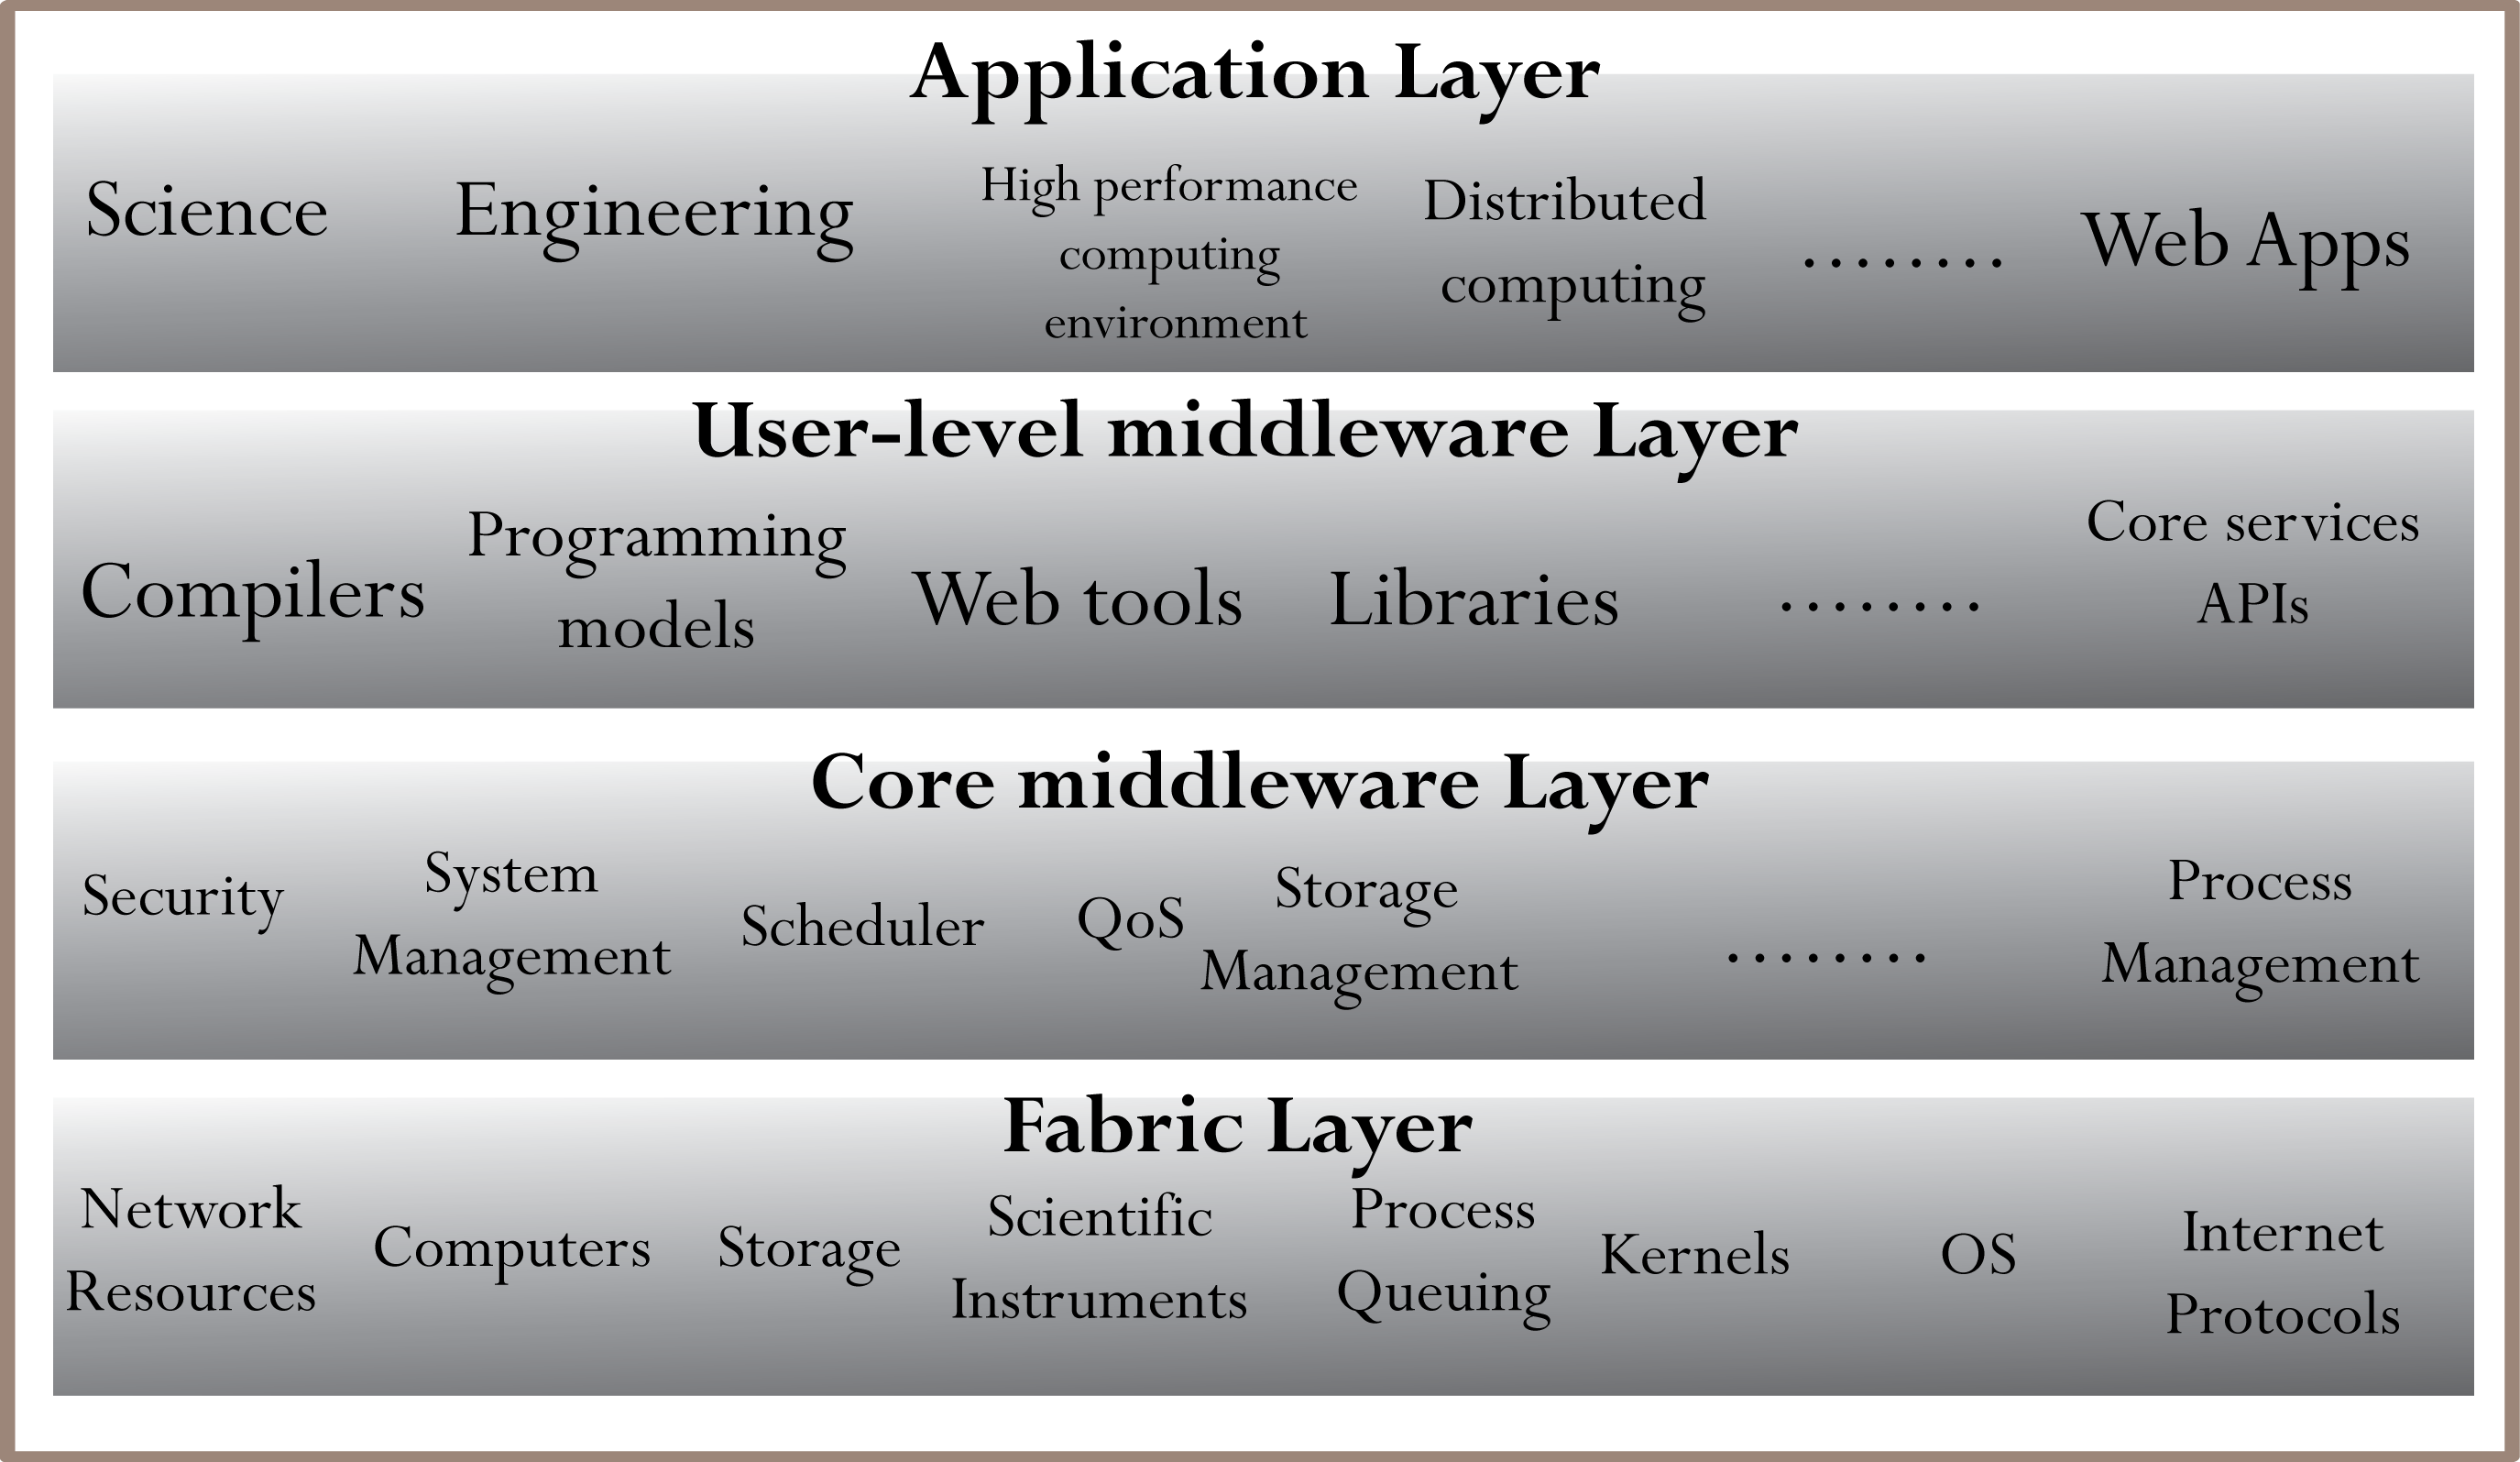
\includegraphics[width=1.0\columnwidth]{architecture}
    \caption{Grid Architecture and components}
	\label{fig:arch}
\end{figure}
\section{Grid Architecture}
Grid architecture \cite{buyya2005gentle} is described in layers, where each layer has some set of functions. Upper layers are application and user centric and lower layers are hardware centric. It consists of four layers i.e., application and portal layer, user-level middleware layer, core middleware layer and fabric layer. Figure~\ref{fig:arch} shows the stack within a grid architecture.
\begin{itemize}
 \item \textbf{Fabric layer:} The lower layer of grid architecture consists of network components, distributed resources, storage devices etc. Computational resources represent multiple architectures such as clusters, supercomputers, servers, ordinary PCs and even PDAs.
 \item \textbf{Core Middleware layer:} The middleware layer is referred to as the ``brains`` behind a computing grid. It provides tools for managing grid elements. It offers services like remote process management, allocation of resources, storage access, resource information registration/discovery, security, and Quality of Service (QoS).
 \item \textbf{User-level Middleware:} This layer helps users to build applications for grid with application development environment and various sets of programming tools. It has access to API's provided by the core middleware layer. 
\item \textbf{Application layer:} This is the layer users interact with. This includes applications in engineering, science, business, finance and more. This also provide development toolkits to support the applications. Grid portals can also offer scalable web-based application services. 
\end{itemize}

\section{Grid job scheduler}
Grid performance can be improved in terms of job processing time by making sure that all the resources available in the grid are utilized optimally using a good job
scheduling algorithm. Job scheduler exists in many conventional distributed environment systems but in grid there are several characteristics that make the scheduling different and more challenging. Some of these characteristics are dynamic structure of the computational grid, high heterogeneity of resources, jobs and interconnection networks, existence of local policies on resources and local schedulers, the large scale of the grid system and security \cite{xhafa2010computational}.\\
The grid scheduler has to follow a series of steps \cite{nabrzyski2004grid} : (1) Collecting information of jobs submitted to the grid, (2) Collecting available resource information, (3) Computation of the mapping of jobs to selected resources, (4) Jobs allocation according to the mapping, and (5) Monitoring of job completion.
There are two types of scheduling :
\begin{itemize}
\item \textbf{Static scheduling:} Jobs are statically assigned to resources before their execution begins. The jobs can not be rescheduled or interrupted once its execution starts.
\item \textbf{Dynamic scheduling:} Re-evaluation is allowed of already taken assignment decisions during job execution is allowed\cite{chtepen2005dynamic} . It can trigger job migration or interruption, based on dynamic information about the status of the system and the workload.
\end{itemize}
The Job scheduling in Grid can be correlated with a classical problem, Flexible Job-shop Scheduling problem(FJSP) \cite{brucker1990job} with dynamic changes of resources and their availability. Besides these grid jobs need to be scheduled as soon as possible after they are enqueued in the job queue, granting the scheduler only a few minutes of time to find the scheduling strategy. FJSP consists of routing subproblem and the scheduling subproblem \cite{wang2012enhanced}. Routing problem is to assign each job with a resource among a set of resources and scheduling problem is to obtain a feasible and satisfactory sequence of jobs within the resources.\\
Computationally, FJSP is as hard as JSP which is an NP Hard problem\cite{garey1979computers} . So finding near optimal solution in polynomial time is our aim. The problem becomes even more interesting when multiple objectives are there to be taken care of.  Nearly all job scheduling algorithms work on single objective like makespan (classical FJSP minimize makespan only).\\
Finding near optimal solution for FJSP problem with more than one objective in a time efficient way is a difficult task. Grid environment being dynamic in nature, reallocation of jobs is quite evident in it. \\
Our approach of solving the above problem using Non-dominated sorting evolutionary algorithm for minimization of multiple objectives, is well enough to find near optimal scheduling strategy in time. The running time complexity of algorithm is $O(GMN^2)$ where $G$ is the number of generations or iterations, $M$ is the number of objectives and $N$ is the population size of the chromosomes or scheduling strategies to run the algorithm.\\

\section{Motivation}
Grid aims at aggregating widely distributed resources and providing low cost computing resources to users. Resources can be computers, storage space, network resources connected through internet or private network with a middleware providing management capability. An Essential part of a Grid system is an efficient scheduling system i.e. resource sharing problem in dynamic and multi-institutional organizations \cite{foster2001anatomy}. Grid scheduling algorithms are inspected with different perspectives, such as static vs. dynamic, application models, QoS constraints, objective functions. Maximum utilization of grid resources is the most cogitated objective in scheduling literatures. However other factors like maintaining QoS constraints, cost effectiveness, energy efficient scheduling were either discussed separately or not acknowledged. Fair amount of importance should be given to user satisfaction, time and cost deadline of jobs. In 2007, Gartner estimated that the Information and Communication Technology industry is liable for 2\% of the global $CO_2$ emission annually, which is equal to that from the aviation industry \cite{pettey2007gartner}. A study done at the Lawrence Berkeley National Laboratory shows that the cooling efficiency (the ratio of computing power to the cooling power) of data centers varies drastically from a low value of 0.6 to a high value of 3.5 \cite{greenberg2006best}. \\
Above mentioned facets clearly show an urgency for a multi-objective grid scheduler, dealing them on their gravity of importance.
\section{Contribution of this thesis}
We present a multi-objective Job scheduler based on an evolutionary algorithm. The aim of this work is to give grid administrators a better scheduler, which will give better grip on the trade off among cost, utilization, energy efficiency and QoS. The scheduler can cope up with the dynamic behavior of resources, resource constraints and predecessor job constraints. A job grouping mechanism is proffered for fine grained jobs. \\
Pareto front approach is taken in multi-objective optimization. Non-dominating sorting mechanism with avant-garde crossover and mutation operator enables the scheduler to explore the search space minutely.\\
Objective functions can be classified into two categories: application-centric and resource-centric. Negotiation and trade off between two types of objectives is necessary. Our generalized multi-objective scheduler provides options to add and remove objective functions.
\section{Organization of the Thesis}
The organization of the rest of the thesis and a brief outline of the chapters
is as follows.
In chapter 2, some related works on job scheduling in grids and their merits and demerits have been discussed.
In chapter 3, Multi-objective Evolution based Dynamic Job Scheduler in Grid has been presented. Here problem definition, job-grouping strategy, problem formulation, MOJS module and algorithms are described.
In Chapter 4, implementation details and experimental results are given.
Chapter 5 sums up the work with conclusion and future work.